\documentclass[12pt,a4paper]{report}

\usepackage[left=2cm, right=2cm, top=4cm, bottom=2cm]{geometry}
\usepackage{enumitem}
\usepackage{fontspec}
\usepackage{tikz}
\usepackage{amsmath}
\usepackage{algpseudocode}

%Eventos
\algblockdefx[Initially]{Initially}{EndInitially}{\textbf{initially do}}{\textbf{end initially}}
\algblockdefx[Upon]{Upon}{EndUpon}[1]{\textbf{upon #1}}{\textbf{end upon}}

\begin{document}
	%Portada
	\begin{titlepage}
		\centering
		{\scshape\LARGE Universidad Nacional Autónoma de México \par}
		\vspace{1cm}
		{\scshape\Large Computación Distribuida\par}
		\vspace{1.5cm}
		{\huge\bfseries Tarea 7\par}
		\vspace{.5cm}
		{\Large\itshape Edgar Quiroz Castañeda \par}
		\vspace{.5cm}
		{\Large\itshape Jerónimo Almeida Rodríguez \par}
		\vfill
		 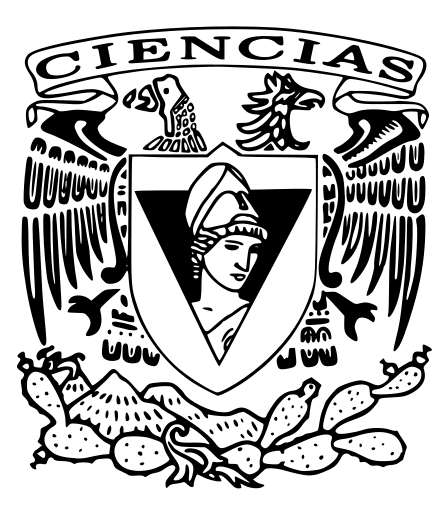
\includegraphics[width=0.5\textwidth]{escudo_f-ciencias.png}
		\vfill

		{\large Jueves 1 de noviembre del 2018 \par}
	\end{titlepage}

	\pagebreak
	\setlength{\voffset}{-0.75in}
	\setlength{\headsep}{5pt}

	%Ejercicios
	\begin{enumerate}
		%1
		\item {
			Considera la ejecución $\alpha$ de la Figura 1. Los retardos máximos
			para cada uno de los eventos son $B_{i, j}$, donde $i$ es el evento
			que envía y $j$ el que recibe.
			\begin{enumerate}
				%a
				\item {
					¿Cuánto vale el retardo máximo de $c$ a $e$ en términos de
					las $B$s? Es decir, dado $real(c)-real(e) \leq x$, ¿cuánto
					vale $x$?\\
					Sólo existe un camino dirigido de $c$ a $e$, por lo que la
					cota está dada únicamente por los retardos máximos de las
					aristas de ese camino.
					$x = B_{cd} + B_{de}$
				}

				%b
				\item {
					Anotar los eventos con los relojes escalares y los relojes
					vectoriales.\\
					Suponinendo que el mensaje de $a$ a $e$ es lo último en
					llegar.\\
					Reloj escalar\\
					\begin{tabular}{| c | c | c | c |}
						\hline
  						tiempo & $P_0$ & $P_1$ & $P_2$ \\ \hline
  						 1 & 1 & 0 & 0\\ \hline
  						 2 & 1 & 2 & 0\\ \hline
						 3 & 1 & 3 & 0\\ \hline
						 4 & 1 & 3 & 4\\ \hline
						 5 & 1 & 3 & 5\\ \hline
						 6 & 1 & 6 & 5\\ \hline
						 7 & 1 & 7 & 5\\ \hline
						 8 & 8 & 7 & 5\\ \hline
						 9 & 9 & 7 & 5\\ \hline

						\hline
					\end{tabular}\\
					Reloj vectorial\\
					\begin{tabular}{| c | c | c | c |}
						\hline
  						tiempo & $P_0$ & $P_1$ & $P_2$ \\ \hline
  						 1 & (1, 0 ,0) & (0, 0 ,0) & (0, 0 ,0)\\ \hline
  						 2 & (1, 0 ,0) & (1, 1 ,0) & (0, 0 ,0)\\ \hline
						 3 & (1, 0 ,0) & (1, 2 ,0) & (0, 0 ,0)\\ \hline
						 4 & (1, 0 ,0) & (1, 2 ,0) & (1, 2 ,1)\\ \hline
						 5 & (1, 0 ,0) & (1, 2 ,0) & (1, 2 ,2)\\ \hline
						 6 & (1, 0 ,0) & (1, 3 ,2) & (1, 2 ,2)\\ \hline
						 7 & (1, 0 ,0) & (1, 4 ,2) & (1, 2 ,2)\\ \hline
						 8 & (2, 4 ,2) & (1, 4 ,2) & (1, 2 ,2)\\ \hline
						 9 & (3, 4 ,2) & (1, 4 ,2) & (1, 2 ,2)\\ \hline

						\hline
					\end{tabular}
				}

				%c
				\item {
					¿Cuáles son eventos concurrentes y cuáles no?\\
					Existe una trayectoria que pasa por todos los eventos, por
					lo que para todo par de eventos, alguno de ellos causó al
					otro. Entonces no hay eventos concurrentes.
				}

				%d
				\item {
					Describe todos los cortes consistentes de $\alpha$.\\
					Dígamos que $a$ está en alguno de los dos conjuntos. \\
					Entonces ni $b$ ni $e$ pueden estar es ese mismo conjunto,
					por lo que ambos están en el otro. \\
					Esto implica que $c$ y $d$ tienen que estar en el mismo
					conjunto que $a$. \\
					Pero hay un arco que va de $c$ a $d$, por lo que no pueden
					estar en el mismo conjunto. \\
					Pero por construcción esta configuración es la única que
					evita conflictos entre $a$, $e$ y $b$.\\
					Entonces, no hay cortes consistentes de $\alpha$.
				}
			\end{enumerate}
		}

		%2
		\item {
			Sea $G = (V, E)$ la gráfica dirigida de causalidad de una ejecución
			$\alpha$, $e, e' \in V$ y $L$ un reloj vectorial.\\
			Un evento causó a otro si existe un camino dirigido que inicia en
			el primer evento y acaba en el segundo.\\
			Demuestra que $e$ causó a $e'$ si y sólo si $L(e) < L(e')$.
		}

		%3
		\item {
			Lee los primeros 5 sueños del libro \textit{Einstein's Dream}.
			Redacta un pequeño resumen de cada uno de ellos.
		}

		%4
		\item {
			Sean $A$ y $B$ dos procesos cuyos relojes no están sincronizados,
			pero ambos tienen un $drift$ acotado. Un mensaje de $A$ a $B$
			tarda a lo más $D$, en tiempo real.\\
			Propón un algoritmo para que $B$ estime el tiempo de llegada de un
			mensaje de $A$, si este manda mensajes cada $T$ unidades de tiempo.\\
			La idea es iniciar con una estimación mínima de cuando va a llegar
			el próximo mensaje, y si el tiempo real es mayor a la estimación,
			entonces se actualiza la estimación.\\
			Cómo el $drfit$ está acotado, entonces eventualmente se llegará a
			un retardo máximo para la estimación.

			\begin{algorithmic}[1]
				\Initially
				 	\State maxDelay = 1
					\State lastSeen = 0
					\State suspecting = false
				\EndInitially
				\Statex

				\Upon{receiving $m$ from $A$}
					\If{suspecting}
						\State suspecting = false
						\State maxDelay = clock.curretTime()-lastSeen
						\State print("no longer suspecting")
					\EndIf
					\State lastSeen = getTime()
					\State print("next message at most at", getTime() + maxDelay)
				\EndUpon
				\Statex

				\Upon{$maxDelay < clock.curretTime()-lastSeen$}
					\State suspecting = true
					\State print("suspecting from process A")
				\EndUpon
			\end{algorithmic}
		}
	\end{enumerate}

\end{document}
